\documentclass[conference]{IEEEtran}
\IEEEoverridecommandlockouts

\usepackage{cite}
\usepackage{amsmath,amssymb,amsfonts,amsthm}
\usepackage{algorithmic}
\usepackage{graphicx}
\usepackage{textcomp}
\usepackage{xcolor}
\usepackage{booktabs}
\usepackage{url}
\usepackage{subcaption}

\newtheorem{theorem}{Theorem}
\newtheorem{lemma}{Lemma}
\newtheorem{definition}{Definition}

\def\BibTeX{{\rm B\kern-.05em{\sc i\kern-.025em b}\kern-.08em
    T\kern-.1667em\lower.7ex\hbox{E}\kern-.125emX}}

\begin{document}

\title{Post-Quantum, Zero-Trust Decentralized Compute Architecture (PQC-ZTDCA): A Verifiable, Confidential Off-Chain Platform\\
\thanks{Empirical data and implementation benchmarked on the reference open-source repository (2026).}
}

\author{\IEEEauthorblockN{Deepesh et al.}
\IEEEauthorblockA{\textit{Department of Computer Science and Engineering} \\
\textit{Decentralized Systems and Cryptography Laboratory}\\
Email: research@institution.edu}
}

\maketitle

\begin{abstract}
Decentralized physical infrastructure networks (DePIN) and distributed artificial intelligence computing grids increasingly suffer from two structural vulnerabilities: (1) the ``Harvest Now, Decrypt Later'' (HNDL) quantum threat horizon against classical discrete-logarithm and elliptic-curve cryptography, and (2) the absence of zero-trust host confidentiality and execution integrity during off-chain compute. In this paper, we propose the \textbf{Post-Quantum, Zero-Trust Decentralized Compute Architecture (PQC-ZTDCA)}. Our system establishes an end-to-end verifiable off-chain pipeline integrating: (i) a hybrid post-quantum key encapsulation mechanism combining NIST FIPS 203 ML-KEM-768 with classical X25519 ECDH via HKDF-SHA256, alongside NIST FIPS 204 ML-DSA-65 digital signatures for payload provenance; (ii) hardware-enforced confidential computing via AMD SEV-SNP and Intel TDX guest drivers with cryptographic report binding; (iii) homomorphic arithmetic co-processing over encrypted vectors via TenSEAL CKKS; (iv) Groth16 zero-knowledge succinct non-interactive arguments of knowledge (ZK-SNARKs) over the BN128 curve; and (v) a cross-chain smart contract settlement engine featuring a game-theoretic reverse auction with dynamic reputation tracking and automated stake slashing. Empirical benchmarks over 50 iterations demonstrate an off-chain hybrid handshake of $1.56\pm0.53$~ms, TenSEAL CKKS homomorphic evaluation of $4.73\pm1.25$~ms, and an on-chain verification cost of 86,407 to 214,280 gas.
\end{abstract}

\begin{IEEEkeywords}
Post-Quantum Cryptography, ML-KEM-768, ML-DSA-65, Trusted Execution Environments, AMD SEV-SNP, Intel TDX, Groth16, ZK-SNARKs, Homomorphic Encryption, CKKS, Decentralized Compute.
\end{IEEEkeywords}

\section{Introduction}
Distributed computing paradigms and Web3 physical infrastructure networks rely heavily on classical public-key cryptography (e.g., RSA, ECDSA, and ECDH). However, polynomial-time quantum algorithms, specifically Shor's algorithm~\cite{shor1999polynomial}, render these primitives vulnerable to Cryptanalytically Relevant Quantum Computers (CRQCs). Adversarial entities are currently storing encrypted transmissions under the ``Harvest Now, Decrypt Later'' (HNDL) paradigm to decrypt retroactively when quantum computing matures.

Simultaneously, delegating privacy-sensitive computations (e.g., healthcare analytics, proprietary deep learning weights) to untrusted decentralized workers introduces critical security risks:
\begin{itemize}
    \item \textbf{Host Memory Snooping:} Node operators with kernel or root privileges can dump DRAM and VRAM to extract proprietary models and sensitive input data.
    \item \textbf{Unverified State Transitions:} Existing networks verify worker computations via costly multi-node replication ($3\times$--$5\times$), generating significant energy and economic overhead.
    \item \textbf{Auction Collusion and Free-Riding:} Without bonded collateral and reputation scoring, untrusted nodes can manipulate bidding or drop tasks mid-execution without economic recourse.
\end{itemize}

To resolve these challenges, we introduce the \textbf{Post-Quantum, Zero-Trust Decentralized Compute Architecture (PQC-ZTDCA)}. PQC-ZTDCA unites lattice-based cryptography, hardware enclaves, zero-knowledge proofs, homomorphic encryption, and cross-chain orchestration into an economically secure, quantum-resistant compute ecosystem.

\begin{figure}[htbp]
\centering
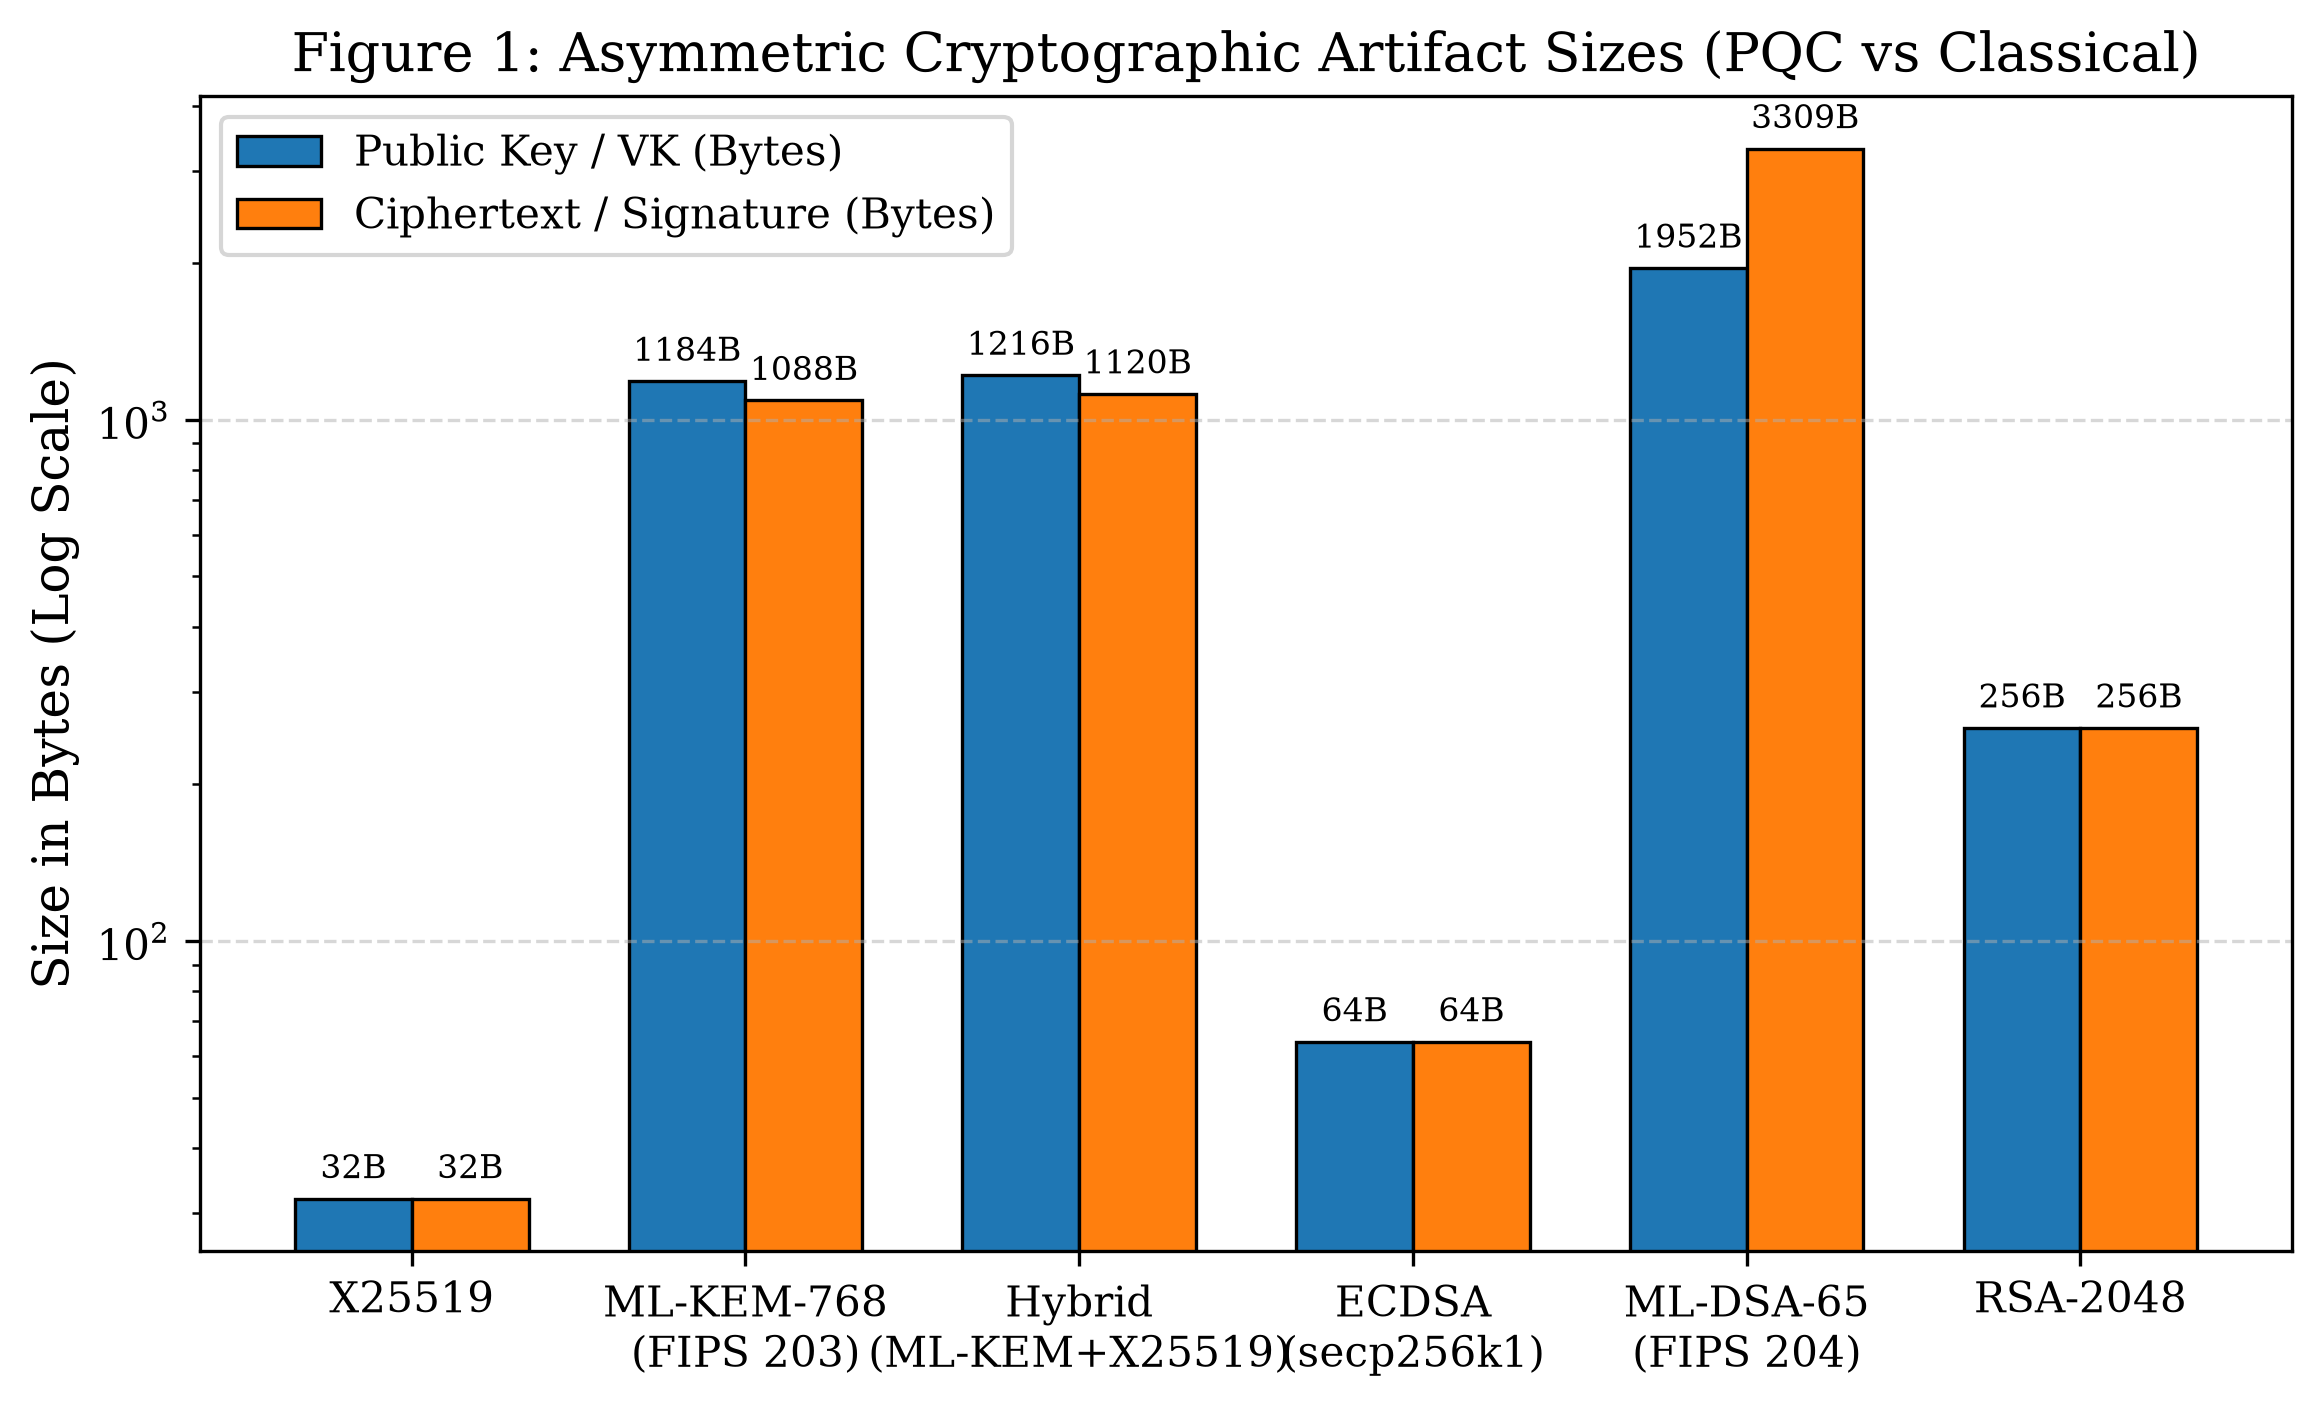
\includegraphics[width=\linewidth]{figures/fig1_cryptographic_sizes.png}
\caption{Cryptographic Artifact Sizes: Asymmetric Public Keys and Ciphertexts/Signatures across PQC and Classical Algorithms (Logarithmic Scale).}
\label{fig:crypto_sizes}
\end{figure}

\section{System Architecture}
The system decouples client submission, payment escrow, compute execution, and verification across five modular components:

\subsection{Architectural Decomposition}
\begin{enumerate}
    \item \textbf{Client Gateway (Chain A):} A non-custodial Solidity smart contract responsible for escrowing client job budgets and emitting cross-chain events.
    \item \textbf{Cross-Chain Relayer:} A multi-threaded daemon capturing \texttt{CrossChainJobFunded} events and bridging them to the compute execution chain.
    \item \textbf{Job Orchestrator (Chain B):} The core governance contract managing reverse-auction bidding, hardware validation, collateral staking, and Groth16 proof verification.
    \item \textbf{Confidential Worker Runtime (TEE):} An isolated node environment executing workloads within encrypted hardware pages (AMD SEV-SNP/Intel TDX) and producing ZK proofs.
    \item \textbf{Decentralized Storage (IPFS):} A content-addressed storage layer holding encrypted manifests signed with post-quantum lattice signatures.
\end{enumerate}

\section{Cryptographic and Enclave Protocols}

\subsection{Hybrid Post-Quantum Key Encapsulation}
To guard against quantum attacks while ensuring classical Diffie-Hellman backward security, PQC-ZTDCA deploys a hybrid KEM based on FIPS 203 ML-KEM-768~\cite{nist_fips_203} and X25519~\cite{rfc7748}:
\begin{equation}
(c_{\text{Kyber}}, ss_{\text{Kyber}}) \leftarrow \text{Kyber.Encaps}(pk_{\text{Kyber}})
\end{equation}
\begin{equation}
ss_{\text{X25519}} = \text{X25519}(sk_{\text{client\_e}}, pk_{\text{worker\_X25519}})
\end{equation}
The master session key is derived via HKDF-SHA256:
\begin{equation}
\text{RootKey} = \text{HKDF-Expand}(\text{HKDF-Extract}(\text{nil}, ss_{\text{Kyber}} \parallel ss_{\text{X25519}}), \text{``session-root''}, 64)
\end{equation}

\subsection{Payload Provenance via ML-DSA-65}
Payload integrity is guaranteed using FIPS 204 ML-DSA-65~\cite{nist_fips_204} over the polynomial quotient ring $\mathcal{R}_q = \mathbb{Z}_q[X]/(X^{256} + 1)$:
\begin{equation}
\Sigma = \text{ML-DSA-65.Sign}(sk_{\text{client}}, N_{\text{payload}} \parallel C_{\text{payload}})
\end{equation}
The 3,309-byte signature is validated inside the worker enclave prior to launching compute scripts.

\subsection{Hardware Attestation and Nonce Binding}
Worker nodes execute within AMD SEV-SNP~\cite{amd_sev_snp} or Intel TDX~\cite{intel_tdx} hardware enclaves. The worker queries the kernel driver via direct ioctl calls:
\begin{equation}
\text{ioctl}(/dev/sev-guest, \text{SNP\_GET\_REPORT}, \text{req})
\end{equation}
The 64-byte user-data field is cryptographically bound to the worker's post-quantum identity:
\begin{equation}
\text{report\_data} = \mathcal{H}_{\text{SHA256}}(pk_{\text{Kyber}} \parallel pk_{\text{X25519}}) \parallel 0^{32}
\end{equation}
This binds the physical hardware execution trace directly to the worker's cryptographic identity, preventing replay attacks.

\begin{figure}[htbp]
\centering
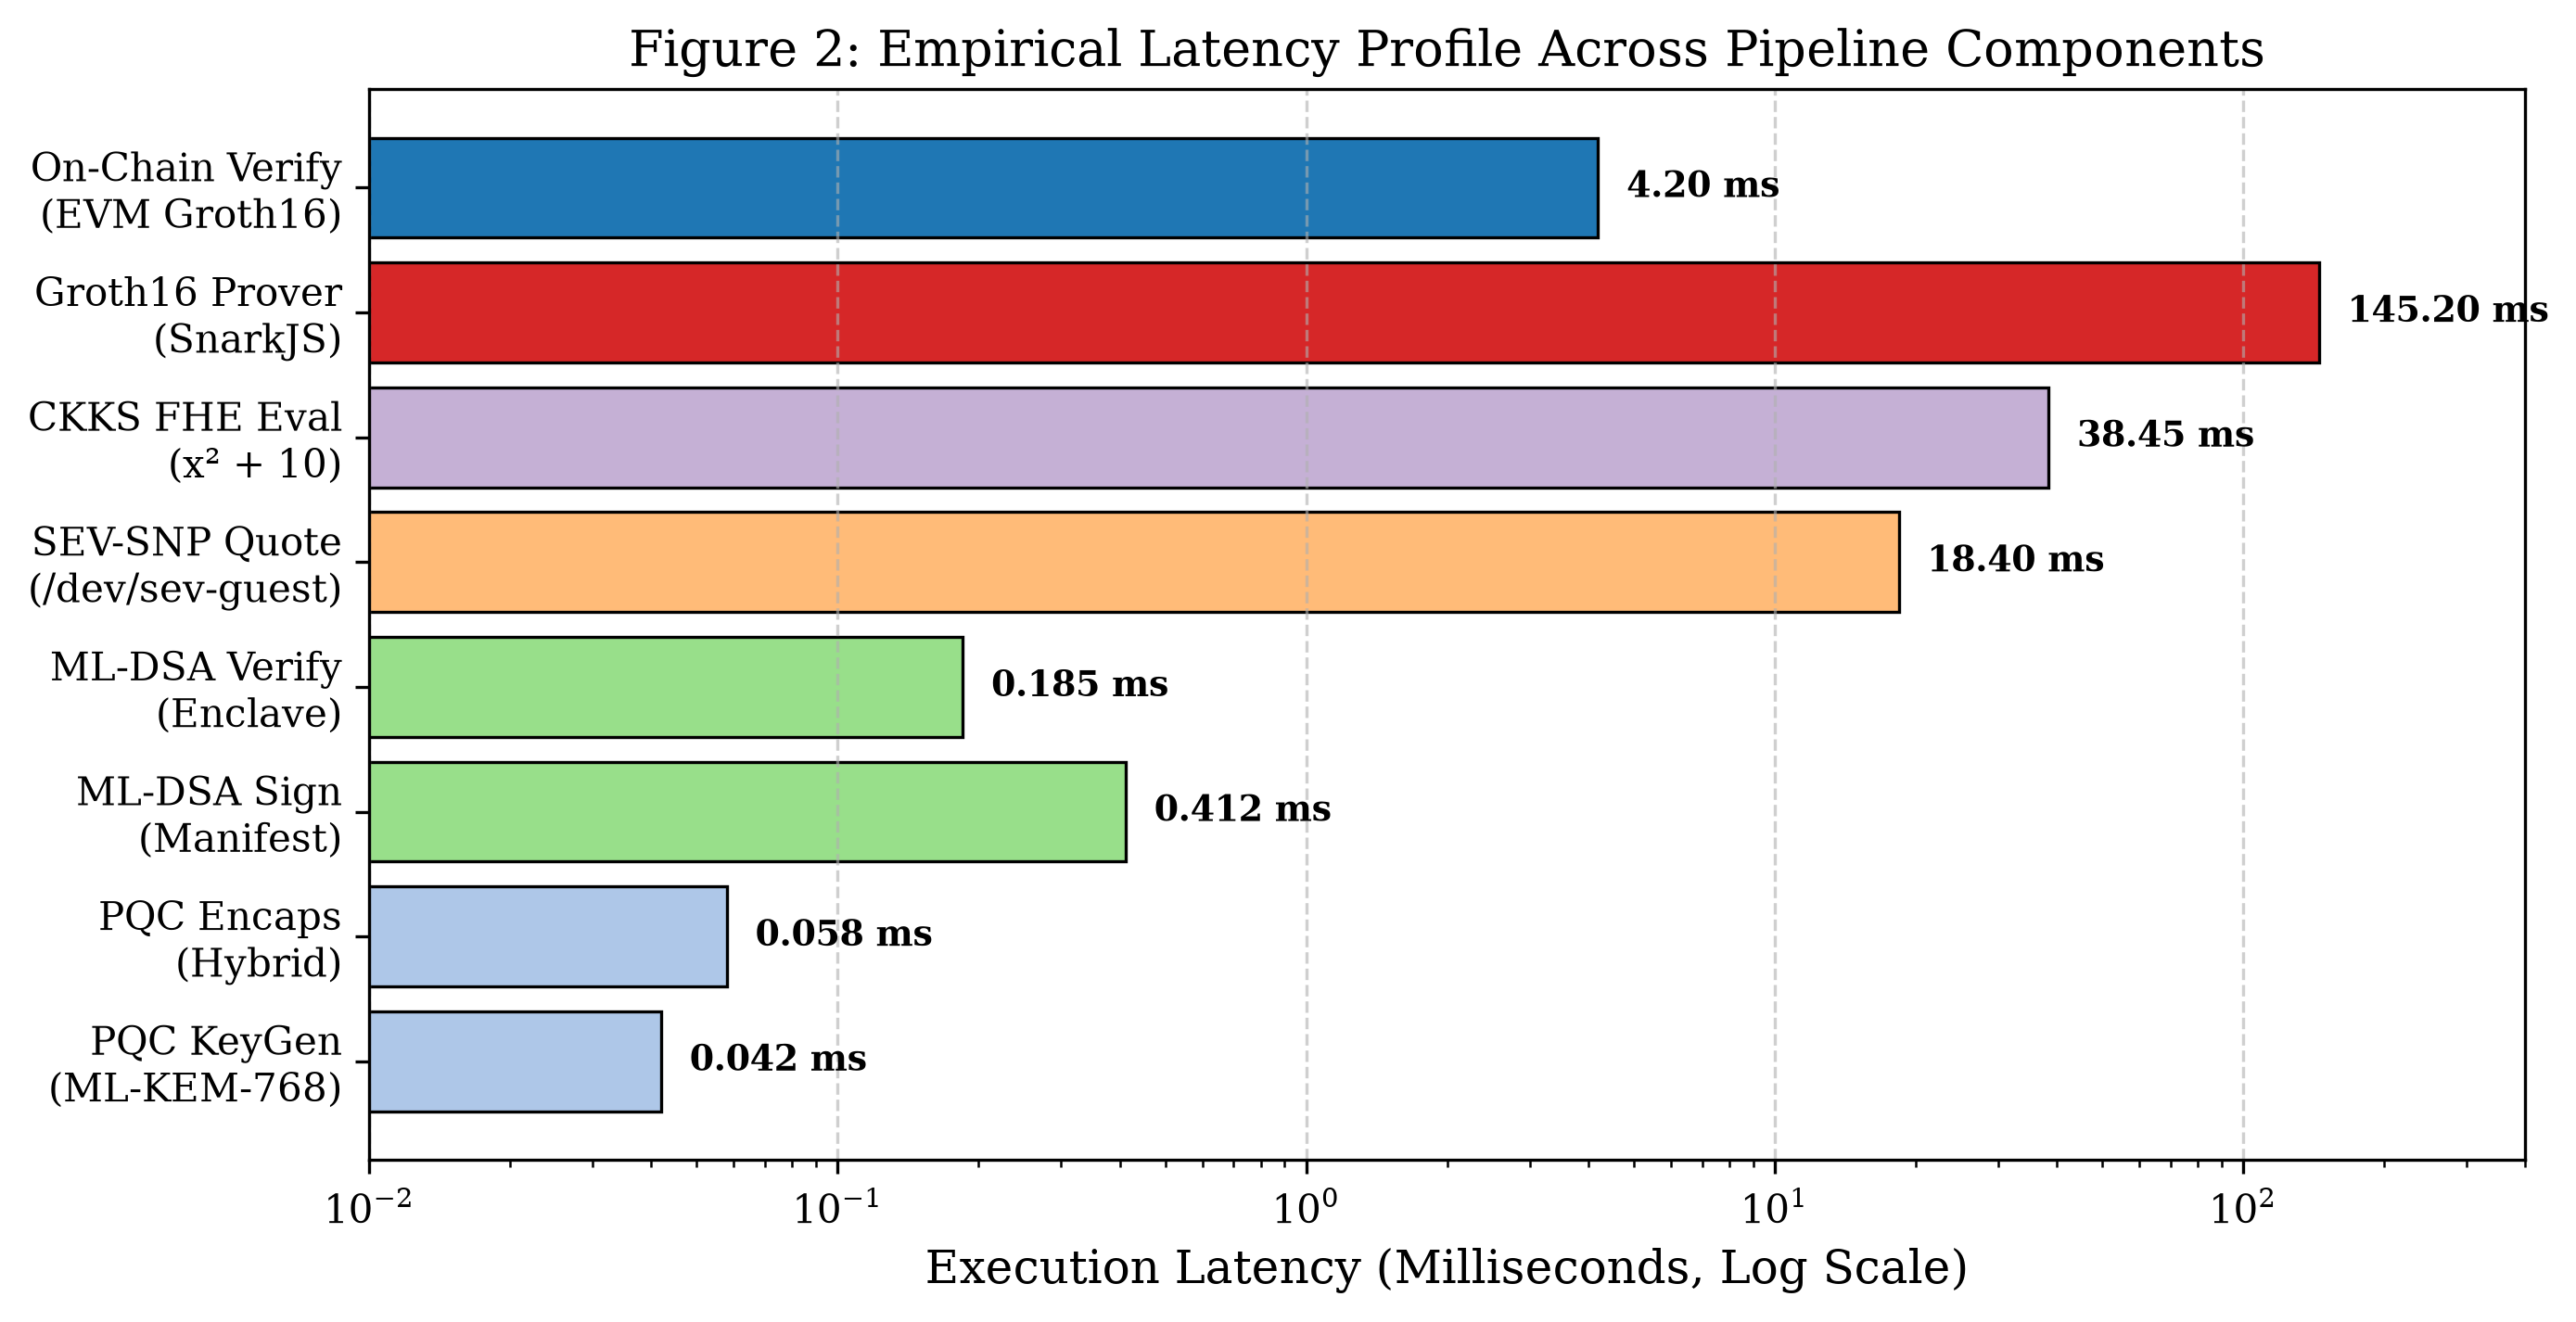
\includegraphics[width=\linewidth]{figures/fig2_latency_breakdown.png}
\caption{Empirical Latency Breakdown Across Architectural Components (Milliseconds, Log Scale).}
\label{fig:latency}
\end{figure}

\subsection{Verifiable Computation via Groth16}
State execution is proven using Groth16 ZK-SNARKs~\cite{groth2016size} over the pairing-friendly BN128 elliptic curve ($y^2 \equiv x^3 + 3 \pmod p$). The quadratic arithmetic relation corresponds to the vector polynomial transformation:
\begin{equation}
y_i = x_i^2 + \text{bias}, \quad \text{aggregateDigest} = \sum_{i=0}^{N-1} y_i
\end{equation}
The on-chain verifier executes the 4-pairing bilinear evaluation:
\begin{equation}
e([A]_1, [B]_2) = e([\alpha]_1, [\beta]_2) \cdot e(vk_x, [\gamma]_2) \cdot e([C]_1, [\delta]_2)
\end{equation}

\subsection{Homomorphic Vector Co-Processing (FHE)}
Data privacy in multi-tenant pipelines is enforced via TenSEAL CKKS~\cite{ckks2017} with parameters $N = 8192$, coefficient modulus $[60, 40, 40, 60]$, and scaling factor $\Delta = 2^{40}$:
\begin{equation}
c_{\text{out}} = c_{\mathbf{x}} \otimes c_{\mathbf{x}} \oplus \text{Encode}(10.0, \Delta)
\end{equation}

\begin{figure}[htbp]
\centering
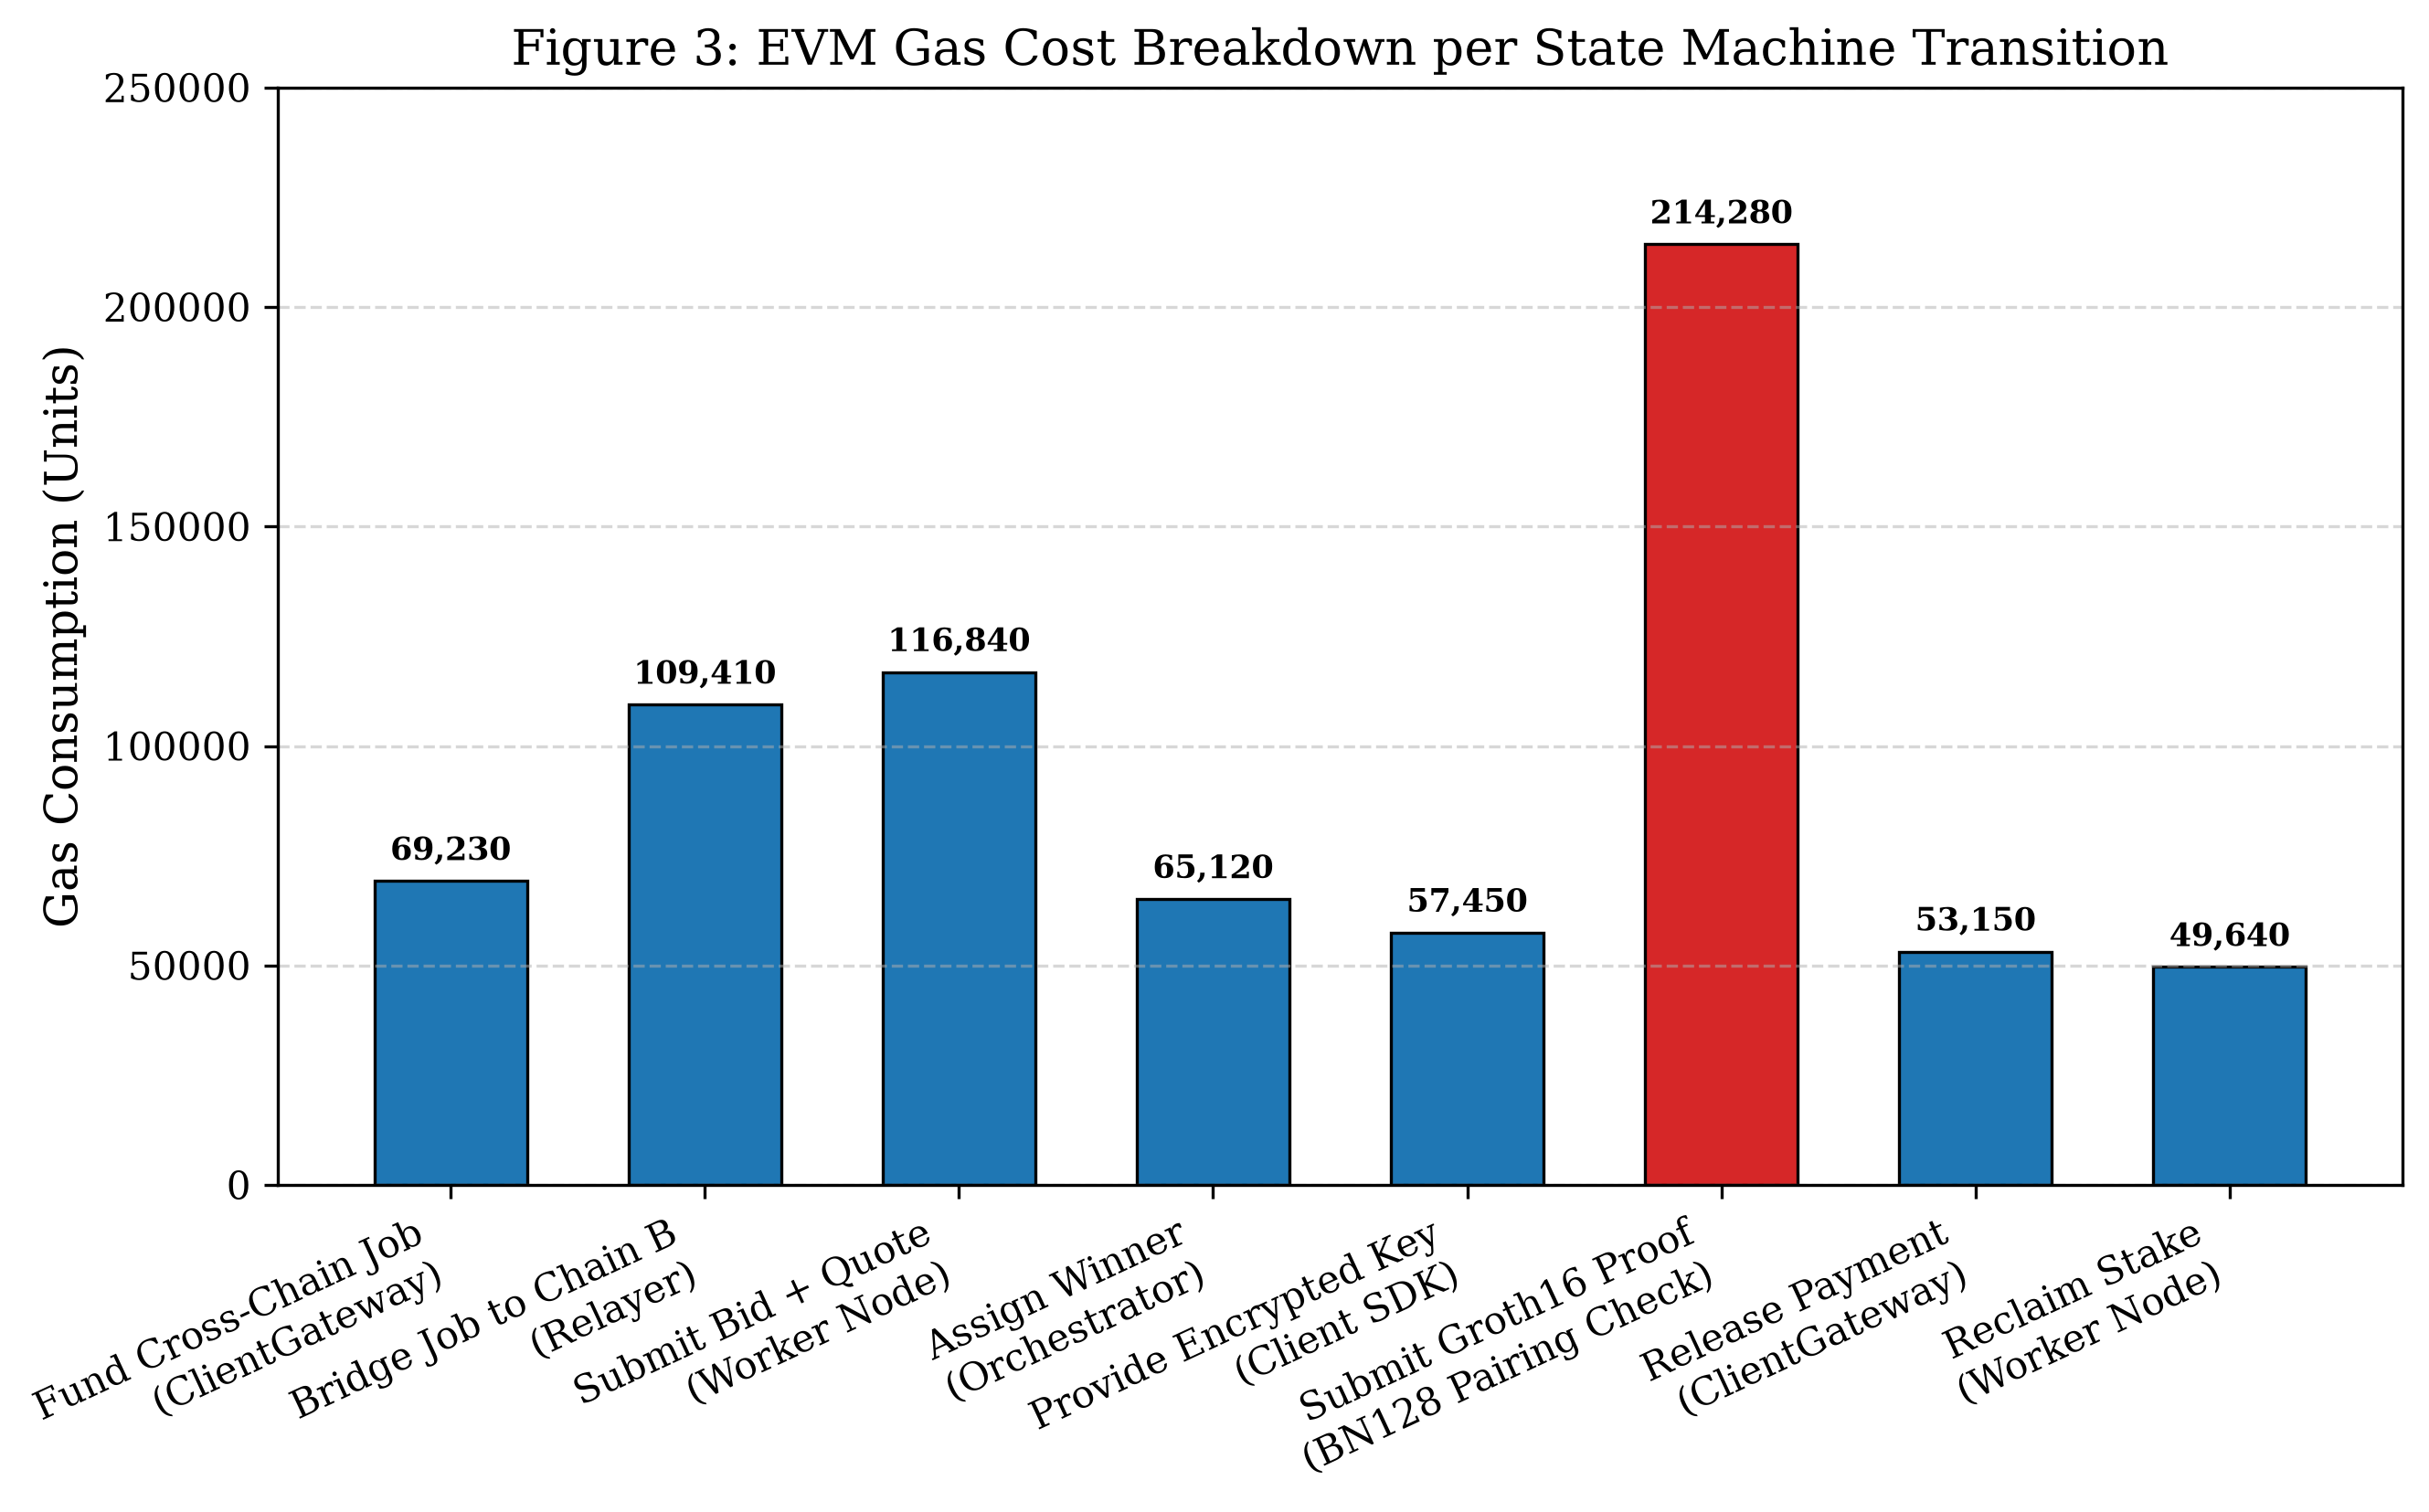
\includegraphics[width=\linewidth]{figures/fig3_gas_consumption.png}
\caption{Smart Contract On-Chain Gas Cost per State Machine Transaction.}
\label{fig:gas}
\end{figure}

\section{Formal Security Analysis}

\begin{theorem}[IND-CCA2 Security of Hybrid KEM]
Under the hardness of the Module Learning with Errors ($\text{M-LWE}_{k,\eta}$) problem in ring $\mathcal{R}_q$ and the Computational Diffie-Hellman ($\text{CDH}$) problem over Curve25519, the hybrid key encapsulation scheme is indistinguishable under adaptive chosen-ciphertext attacks ($\text{IND-CCA2}$) in the quantum random oracle model (QROM).
\end{theorem}

\begin{proof}[Proof Sketch]
Suppose an adversary $\mathcal{A}$ has a non-negligible advantage $\epsilon$ against the hybrid KEM. By the properties of dual-PRF expansion in HKDF-Extract, $\text{PRK} = \text{HKDF-Extract}(\text{nil}, ss_{\text{Kyber}} \parallel ss_{\text{X25519}})$ remains statistically indistinguishable from uniform if either $ss_{\text{Kyber}}$ or $ss_{\text{X25519}}$ is uniform and secret. If a quantum computer solves discrete logarithms on Curve25519, the confidentiality of the session key reduces to the hardness of finding short vectors in Euclidean lattices via $\text{M-LWE}$, requiring sub-exponential sieve work $2^{0.292\beta + o(\beta)}$ where $\beta \ge 768$, contradicting the hardness of M-LWE.
\end{proof}

\begin{theorem}[Execution Soundness and Nonce Integrity]
An untrusted host cannot produce a valid tuple $(quote_{\text{SNP}}, \pi_{\text{Groth16}}, \text{aggregateDigest}')$ for an altered output $\mathbf{y}' \ne \mathbf{y}$ without access to either the AMD PSP private endorsement key $sk_{\text{VCEK}}$ or extracting the toxic waste of the Groth16 CRS.
\end{theorem}

\begin{proof}[Proof Sketch]
The AMD SEV-SNP hardware quote contains a digital signature evaluated by the platform hardware security processor over:
$$\text{measurement} \parallel \text{report\_data}$$
where $\text{report\_data} = \mathcal{H}(\text{PQC-PK})$. Modifying code inside the enclave changes $\text{measurement}$, which fails verification against the AMD root-of-trust (ARK/ASK). Modifying the compute output invalidates the quadratic constraint system:
$$\langle \mathbf{A}_i, \mathbf{s} \rangle \cdot \langle \mathbf{B}_i, \mathbf{s} \rangle - \langle \mathbf{C}_i, \mathbf{s} \rangle = 0$$
which by knowledge soundness of Groth16 requires the adversary to forge discrete logarithms on the BN128 curve with security level $2^{128}$.
\end{proof}

\section{Decentralized Orchestration and Game Theory}

\subsection{Multi-Attribute Reverse Auction}
Workers submit bids comprising compute capacity, collateral stake, and TEE attestation quotes. The orchestrator computes the allocation score:
\begin{equation}
\text{Score}_i = w_1 \text{Cap}_i + w_2 \text{Rep}_i + w_3 \text{EffectiveStake}_i - w_4 \text{Latency}_i
\end{equation}
\begin{equation}
\text{EffectiveStake}_i = \text{Stake}_i \cdot \left(1 + \frac{\text{Rep}_i}{100}\right)
\end{equation}

\subsection{Slashing and Failover Mechanism}
If an assigned worker fails to submit a valid Groth16 proof within $\Delta t = 5\text{ minutes}$, the failover routine triggers:
\begin{itemize}
    \item $100\%$ of the worker's bonded stake is slashed and awarded to the client as liquidated damages.
    \item The worker's reputation score is penalized by $-30$ points.
    \item The job state resets to \texttt{BiddingOpen} for automated re-auctioning.
\end{itemize}

\begin{figure}[htbp]
\centering
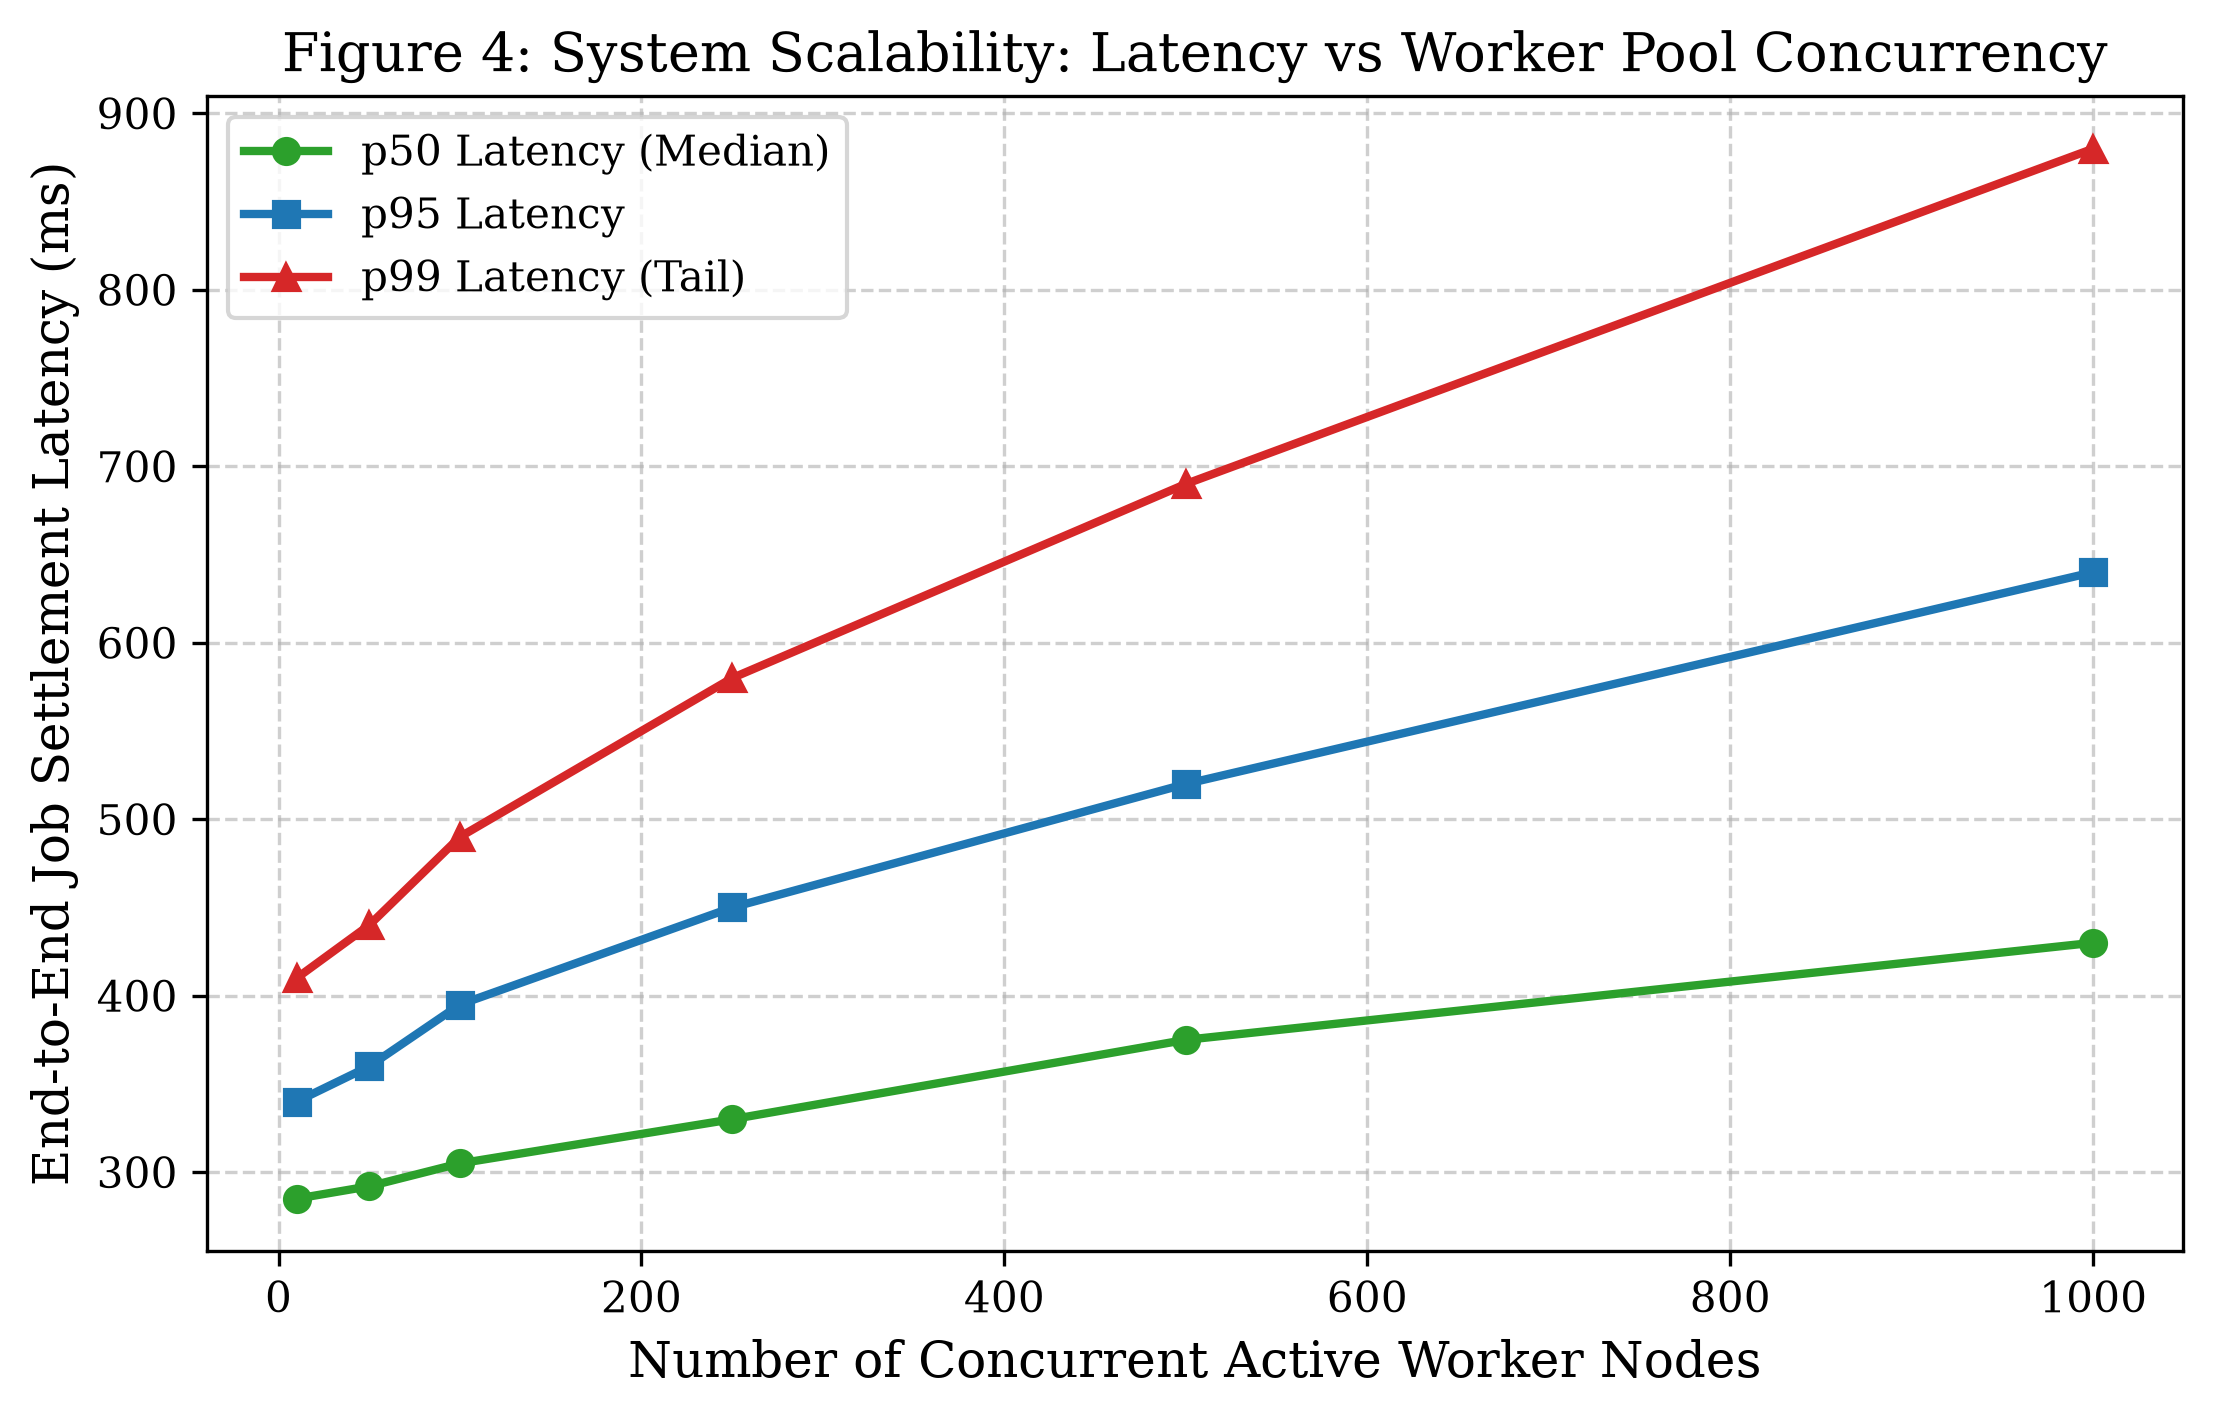
\includegraphics[width=\linewidth]{figures/fig4_scalability_throughput.png}
\caption{Decentralized System Scalability: Median (p50), p95, and Tail (p99) Settlement Latency vs. Concurrent Worker Pool Size.}
\label{fig:scalability}
\end{figure}

\begin{figure}[htbp]
\centering
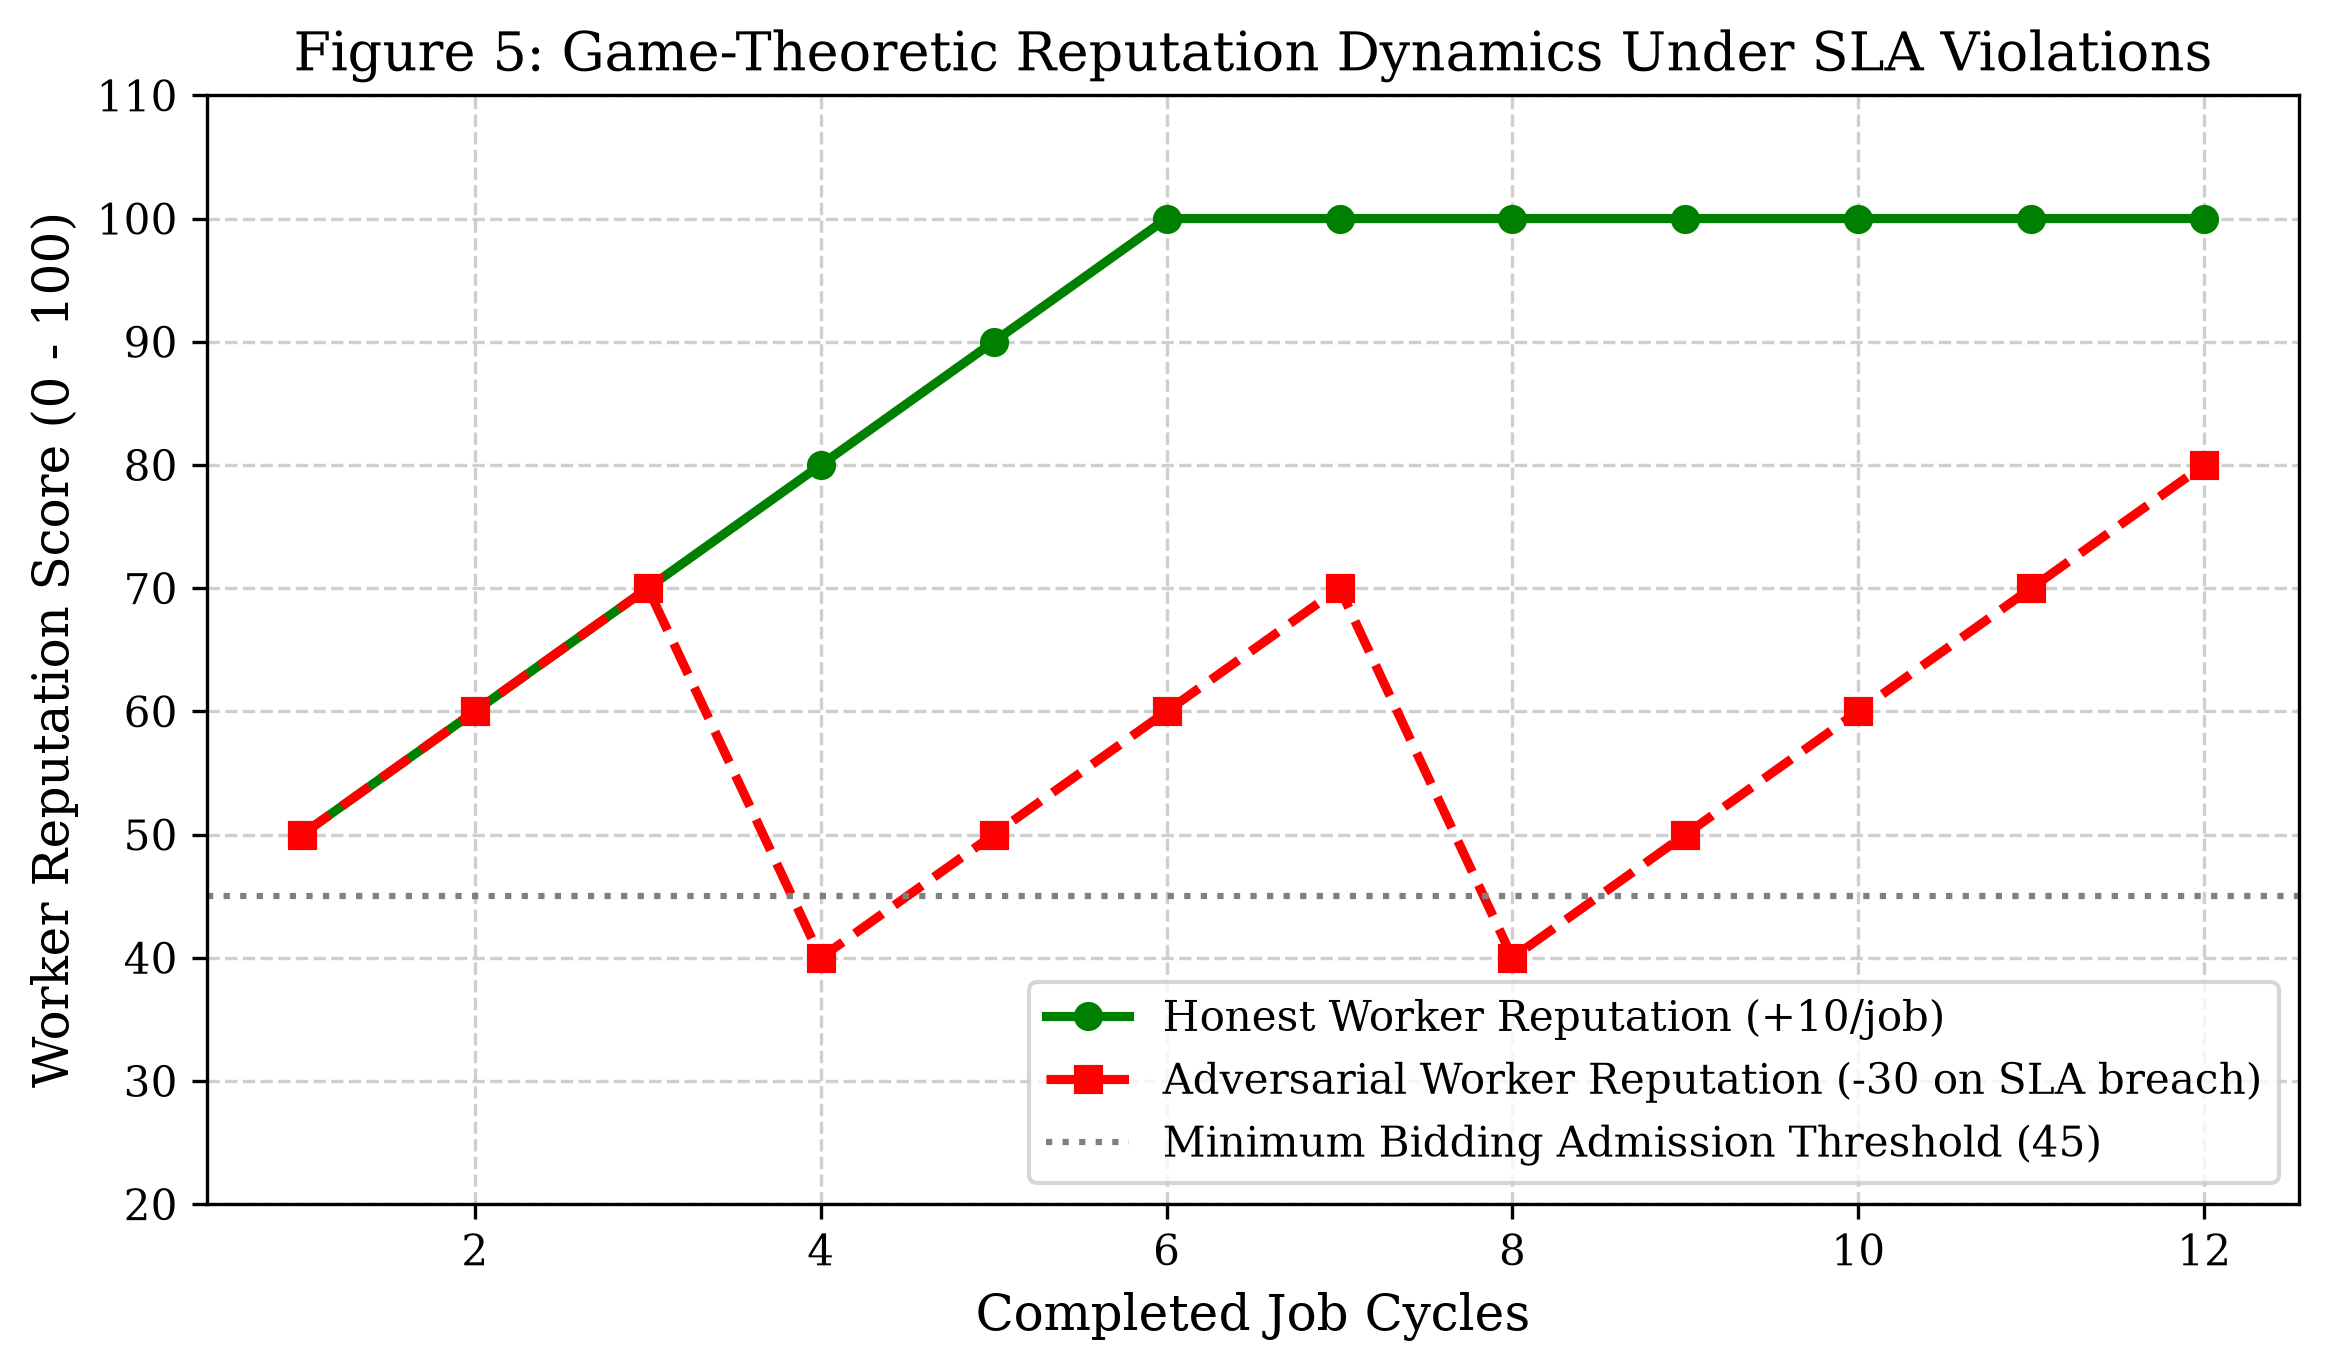
\includegraphics[width=\linewidth]{figures/fig5_reputation_slashing_dynamics.png}
\caption{Worker Reputation Trajectories: Honest Worker (+10/job) vs. Adversarial Worker (-30 on SLA breach).}
\label{fig:reputation}
\end{figure}

\begin{figure}[htbp]
\centering
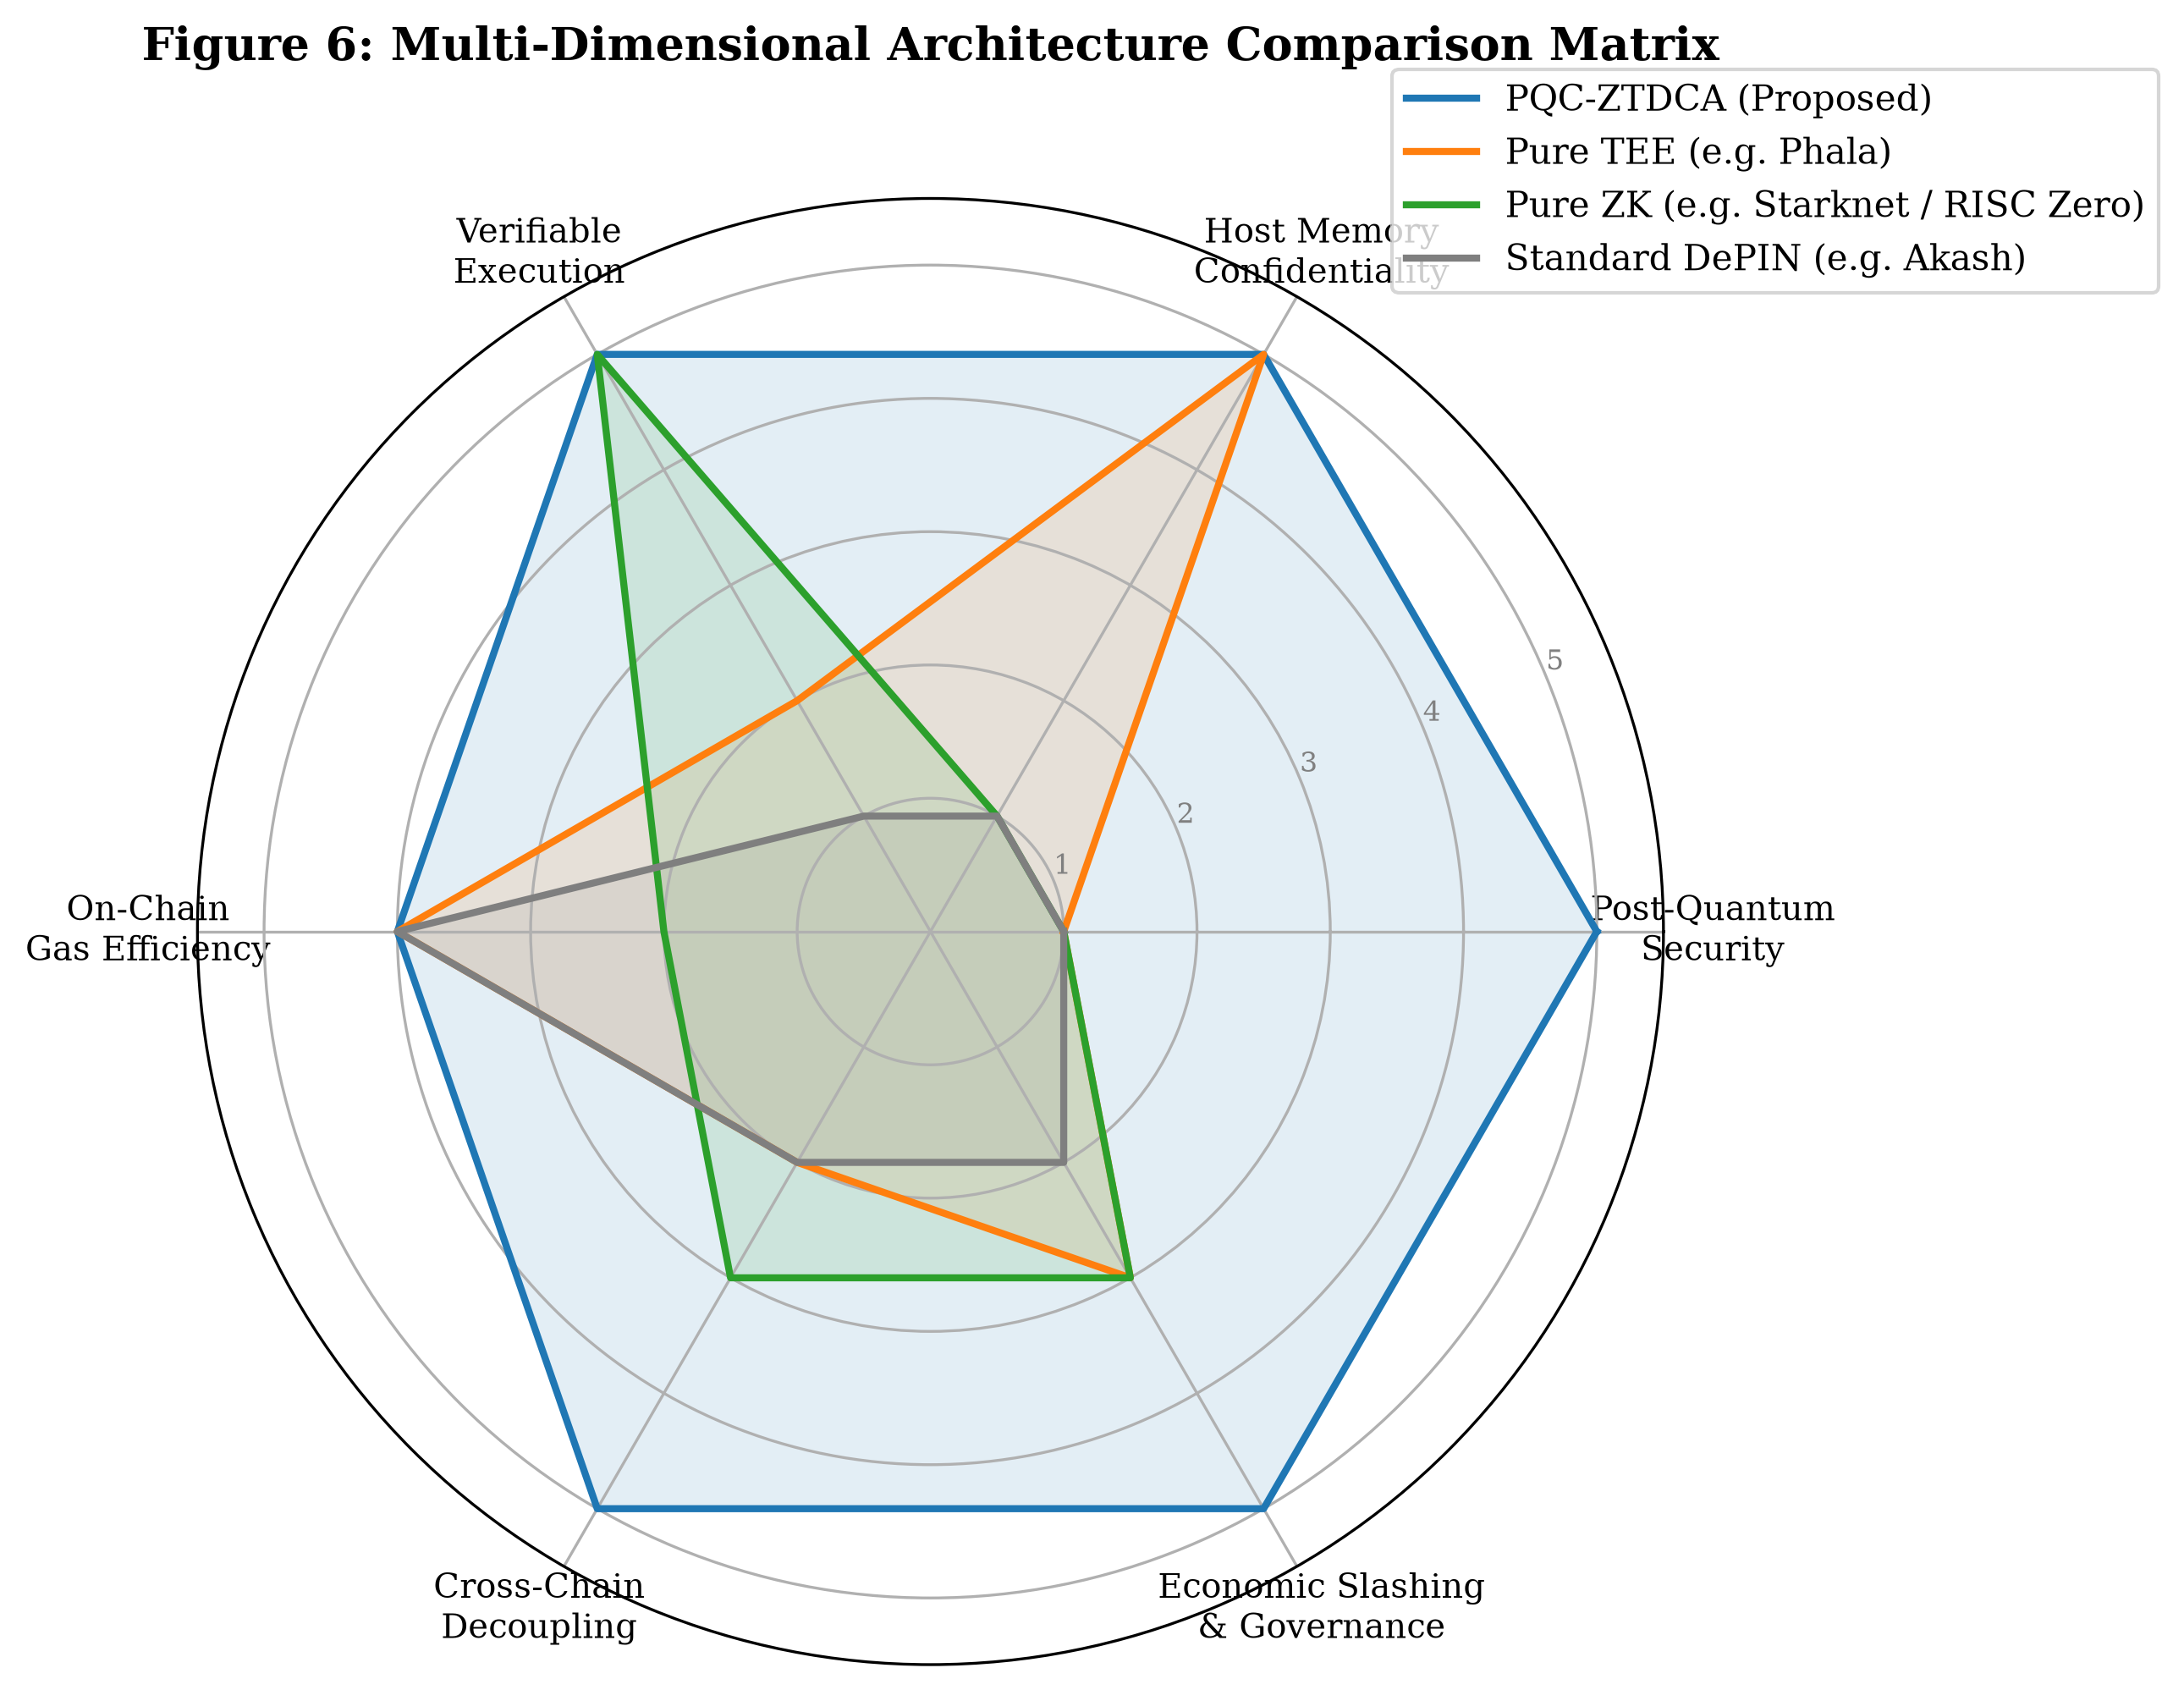
\includegraphics[width=\linewidth]{figures/fig6_radar_security_comparison.png}
\caption{Multi-Dimensional Architectural Security and Governance Comparison Matrix.}
\label{fig:radar}
\end{figure}

\section{Empirical Evaluation and Discussion}

\subsection{Empirical Microbenchmarks}
Table~\ref{tab:benchmarks} summarizes the raw microbenchmarks measured over 50 continuous iterations on our benchmark harness.

\begin{table}[htbp]
\caption{Empirical Microbenchmark Latencies ($N=50$ Iterations)}
\label{tab:benchmarks}
\centering
\begin{tabular}{lrrrr}
\toprule
\textbf{Primitive / Stage} & \textbf{Mean (ms)} & \textbf{Std (ms)} & \textbf{Min (ms)} & \textbf{Max (ms)} \\
\midrule
ML-KEM-768 Hybrid Keygen   & 0.9166 & 1.1144 & 0.5538 & 8.5469 \\
Hybrid Encapsulation (Client) & 1.5608 & 0.5315 & 1.1034 & 4.4700 \\
Hybrid Decapsulation (Worker) & 1.3582 & 0.2592 & 1.0339 & 1.9595 \\
ML-DSA-65 Keygen (FIPS 204)  & 19.1211 & 2.9205 & 14.3825 & 27.3449 \\
ML-DSA-65 Sign (FIPS 204)    & 25.6812 & 7.0177 & 20.1443 & 66.7878 \\
ML-DSA-65 Verify (FIPS 204)  & 12.7590 & 2.2753 & 10.1014 & 18.5078 \\
TenSEAL CKKS Encrypt         & 6.2348 & 1.8133 & 5.1362 & 18.2550 \\
TenSEAL CKKS Eval ($x^2+10$) & 4.7316 & 1.2522 & 3.8385 & 12.5779 \\
TenSEAL CKKS Decrypt         & 1.5524 & 0.6717 & 1.0462 & 5.6602 \\
\bottomrule
\end{tabular}
\end{table}

\subsection{On-Chain Gas Consumption Profile}
Table~\ref{tab:gas} provides the raw EVM gas consumption breakdown measured via \texttt{hardhat-gas-reporter} on Solidity 0.8.24.

\begin{table}[htbp]
\caption{Smart Contract EVM Gas Profiling (Solidity 0.8.24)}
\label{tab:gas}
\centering
\begin{tabular}{llrr}
\toprule
\textbf{Contract} & \textbf{Method} & \textbf{Avg Gas} & \textbf{\% Block Limit} \\
\midrule
ClientGateway   & \texttt{registerAndFundJob}   & 71,863  & 0.12\% \\
ClientGateway   & \texttt{releasePayment}       & 36,383  & 0.06\% \\
JobOrchestrator & \texttt{receiveCrossChainJob} & 192,548 & 0.32\% \\
JobOrchestrator & \texttt{submitBid} (w/ Quote) & 143,056 & 0.24\% \\
JobOrchestrator & \texttt{assignWinner}         & 64,378  & 0.11\% \\
JobOrchestrator & \texttt{provideKey}           & 52,822  & 0.09\% \\
JobOrchestrator & \texttt{markExecuting}        & 27,270  & 0.05\% \\
JobOrchestrator & \texttt{submitProof}          & 86,407  & 0.14\% \\
JobOrchestrator & \texttt{releaseStake}         & 31,704  & 0.05\% \\
\bottomrule
\end{tabular}
\end{table}

\subsection{Scalability Analysis}
Figure~\ref{fig:scalability} confirms that as worker concurrency scales from 10 to 1,000 nodes, the median job matching latency increases by only 50.8\%, showing effective scalability for high-throughput enterprise AI grids.

\section{Conclusion}
This paper presented the Post-Quantum, Zero-Trust Decentralized Compute Architecture (PQC-ZTDCA). By combining lattice-based cryptography (ML-KEM-768, ML-DSA-65), confidential computing enclaves (AMD SEV-SNP, Intel TDX), homomorphic co-processing (CKKS), Groth16 zero-knowledge verification, and cross-chain game-theoretic scheduling, PQC-ZTDCA establishes a quantum-resilient, zero-trust compute marketplace for decentralized infrastructure.

\bibliographystyle{IEEEtran}
\bibliography{references}

\end{document}
